\chapter{Supplementary Information to \Chapref{Longevity}}%labstudy is the label for chapter 2.
\label{chap:Appendix B}

\section{Additional details of data collection and sources}

\subsection{Flight capability}
Species were categorised as either volant, non-volant or gliders. Most birds, apart from ratites, penguins and some flightless rails, are volant.  All mammals apart from bats are non-volant. We classed mammals as gliders if they regularly use gliding as a means of locomotion and have adaptations that aid their descent e.g., skin flaps.



\subsection{Activity period}

Most animals will be active to some extent at both day and night. Therefore activity period was define using the times when a species is feeding/foraging as this is when they are most likely to be exposed to predation. For example, many bats often fly around their roosts during the day but only leave their roosts to feed at night; therefore such species are classed as nocturnal. We defined species as diurnal, nocturnal, crepuscular or cathemeral by looking for the following key phrases in the literature:

\begin{itemize}
  \item \textbf{Diurnal}: diurnal, active in the day, mainly/predominantly/mostly/generally diurnal or active in the day, crepuscular and diurnal or active in the day, diurnal or active in the day and sometimes/occasionally/infrequently/rarely diurnal or active in the day.
  \item \textbf{Nocturnal}: nocturnal, active at night, mainly/predominantly/mostly/generally nocturnal or active at night, crepuscular and nocturnal or active at night, nocturnal or active at night and sometimes/occasionally/infrequently/rarely diurnal or active in the day.
  \item \textbf{Crepuscular}: crepuscular, active at dusk and dawn, active early morning and evening (not afternoon). Note that crepuscular and diurnal animals are classed as diurnal; crepuscular and nocturnal animals are classed as nocturnal
  \item \textbf{Cathemeral}: cathemeral, diurnal and nocturnal, active any time of the day or night, nocturnal and often/frequently diurnal or active in the day, diurnal and often/frequently nocturnal or active at night.
\end{itemize}

In cases where none of the above keywords were present activity pattern was also defined if all other alternatives could be ruled out, for example species with roosting behaviour described as beginning before sunset and ending only after sunrise can be described as diurnal as it excludes nocturnal, cathemeral and crepuscular daily activity feeding patterns.
  


\subsection{Foraging environment}

Foraging environments were defined as terrestrial, semi-arboreal, arboreal, aerial or aquatic, by looking for the following key phrases in the literature:
\begin{itemize}
\item \textbf{Terrestrial}: terrestrial, feeds at ground-level (including rocky areas), mainly/predominantly/mostly/generally feeds at ground-level, feeds at ground-level and sometimes/occasionally/infrequently/rarely feeds above ground-level. 
\item \textbf{Arboreal}: arboreal, feeds at above ground-level (including trees), mainly/predominantly/mostly/generally feeds at ground-level, feeds at ground-level and sometimes/occasionally/infrequently/rarely feeds above ground-level.
\item \textbf{Semi-arboreal}: semi-arboreal, semi-terrestrial, feeds at above ground-level and at ground-level, feeds at ground-level and often/frequently feeds at above ground-level, feeds at above ground-level and often/frequently feeds at ground-level.
\item \textbf{Aerial}: volant, feeds while flying, mainly/predominantly/mostly/generally aerial forager, aerial forager and sometimes/occasionally/infrequently/rarely feeds at ground-level or above ground-level. Includes insectivorous bats and birds.
\item \textbf{Aquatic}: aquatic, feeds in water, mainly/predominantly/mostly/generally feeds in water, feeds in water and sometimes/occasionally/infrequently/rarely feeds at ground-level or above ground-level. Includes marine birds, ducks, seals and otters. If feeds in both terrestrial and aquatic environments counted as terrestrial.
\end{itemize}


\subsection{Fossoriality}

Species were defined as either fossorial, non-fossorial or semi-fossorial by looking for the following key phrases in the literature:
\begin{itemize}
\item \textbf{Fossorial}: fossorial, lives in burrows and rarely leaves them, mainly/predominantly/mostly/generally fossorial, fossorial and sometimes/occasionally/infrequently active above ground. 
\item \textbf{Non-fossorial}: non-fossorial, terrestrial, mainly/predominantly/mostly/generally terrestrial or non-fossorial, terrestrial or non-fossorial and sometimes/occasionally/infrequently burrows, may excavate shallow scrapes but nothing useful for predator defense, incapable of excavating burrows.
\item \textbf{Semi-fossorial}: semi-fossorial, lives in burrows and leaves them frequently, fossorial and often/frequently active above ground, non-fossorial and often/frequently uses burrows, capable of excavating burrows.
\end{itemize}


\subsection{Chronogram calibration diagnosis}

Following the recommendations of \cite{parham2011best}, our chronogram calibration used the following fossil:


Taxa: \textit{Archerpeton anthracos}

Holotype: RM 12056

Author: Carroll 1964

Phylogeny: \citep{reisz2004molecular}

Epoch: Westphalian A (Canada Nova Scotia)

Age: 318.1 - 314.6 Myr

Dating: International Commission on Stratigraphy 2009


\section{Supplementary tables}

\begin{table}[h]
  \caption[ ]{Table B1. Breakdown of numbers of species in each category included in the analyses. Values under the Sample column represent the number of species with 100 or more available longevity studies. Values under the BMR column represent the number of species with available basal metabolic rate (BMR) data.}
  \label{tbl:Table B1.}
  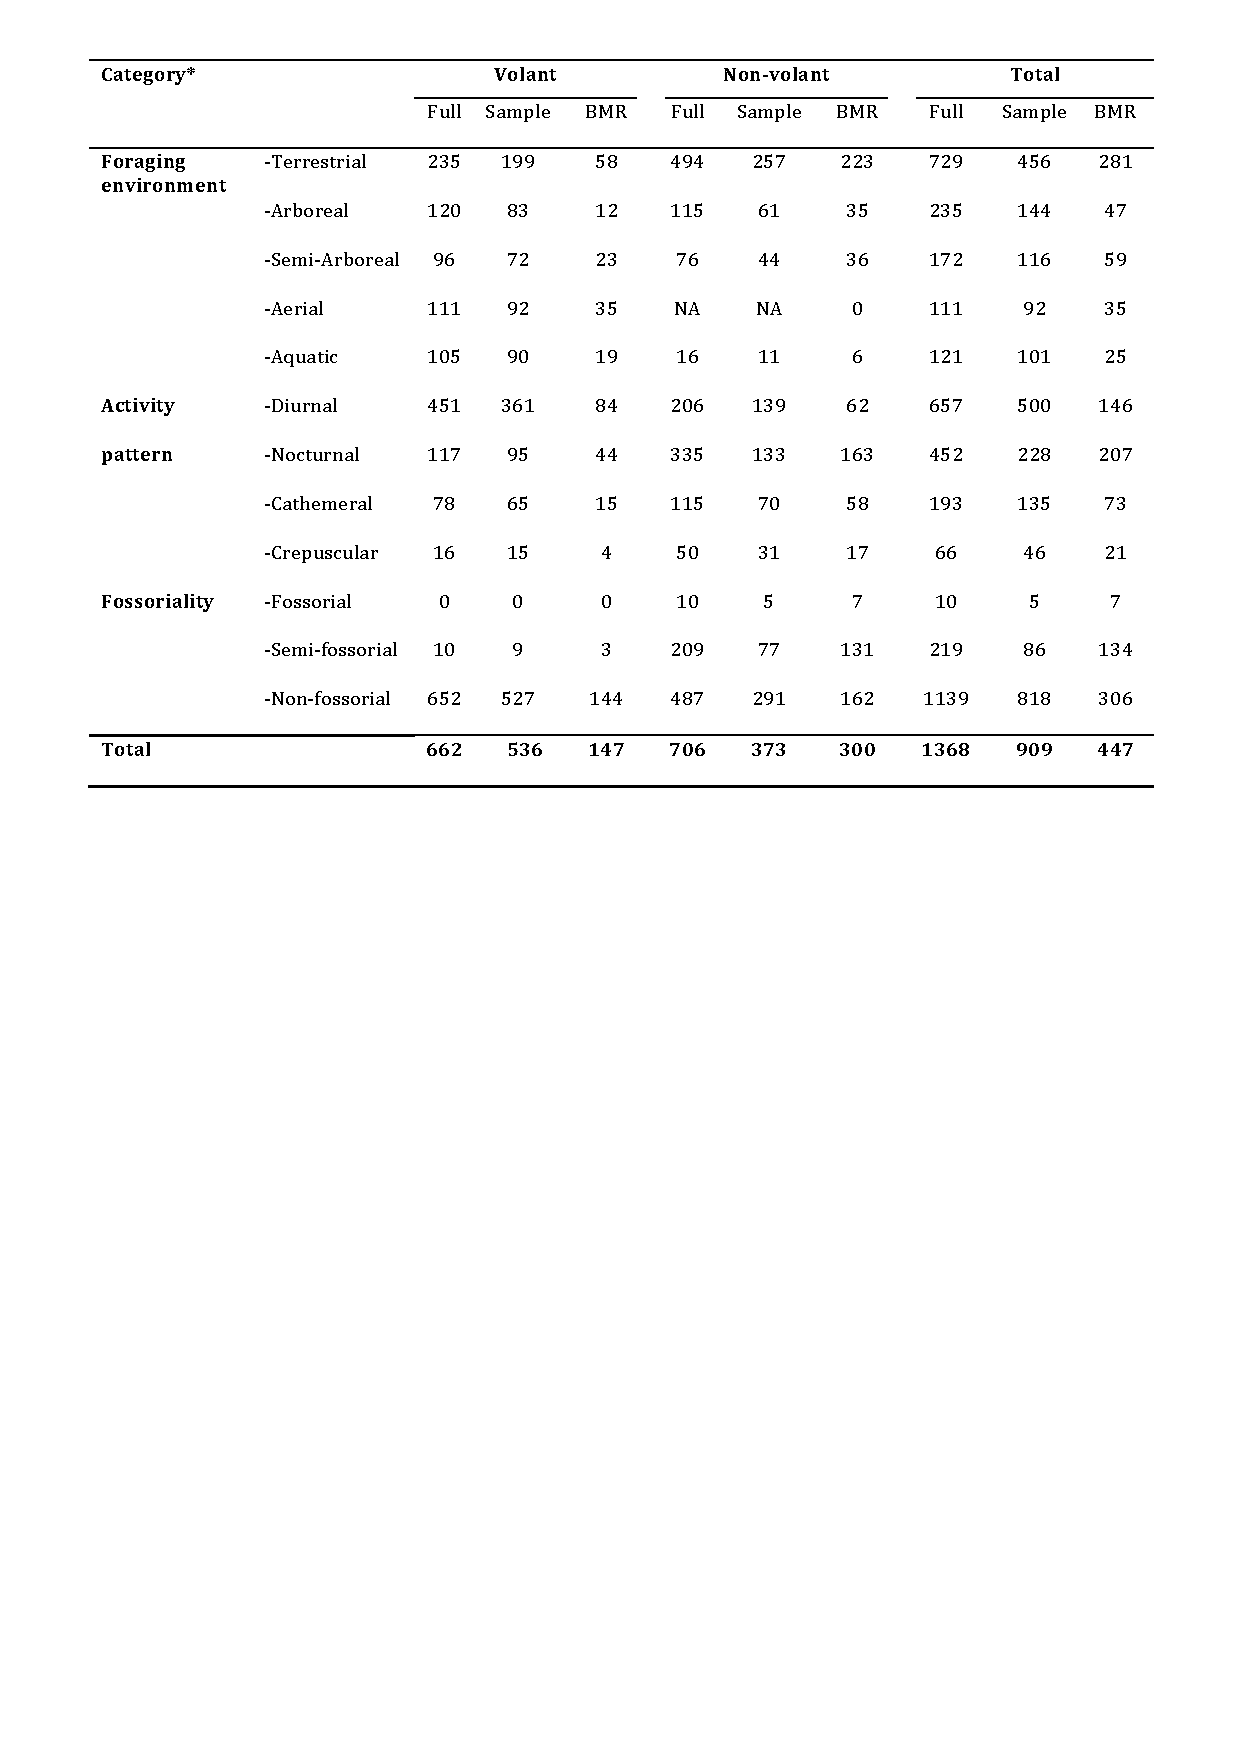
\includegraphics[width=\linewidth]{ch3-longevity-appendix/Table_B1.pdf}
\end{table}


\begin{table}[h]
  \caption[ ]{Table B2: Relationship between maximum longevity (years), body mass (g) and flight capability (volant or non-volant) in 909 species of birds and mammals with over 100 maximum lifespan records.}
  \label{tbl:Table B2.}
  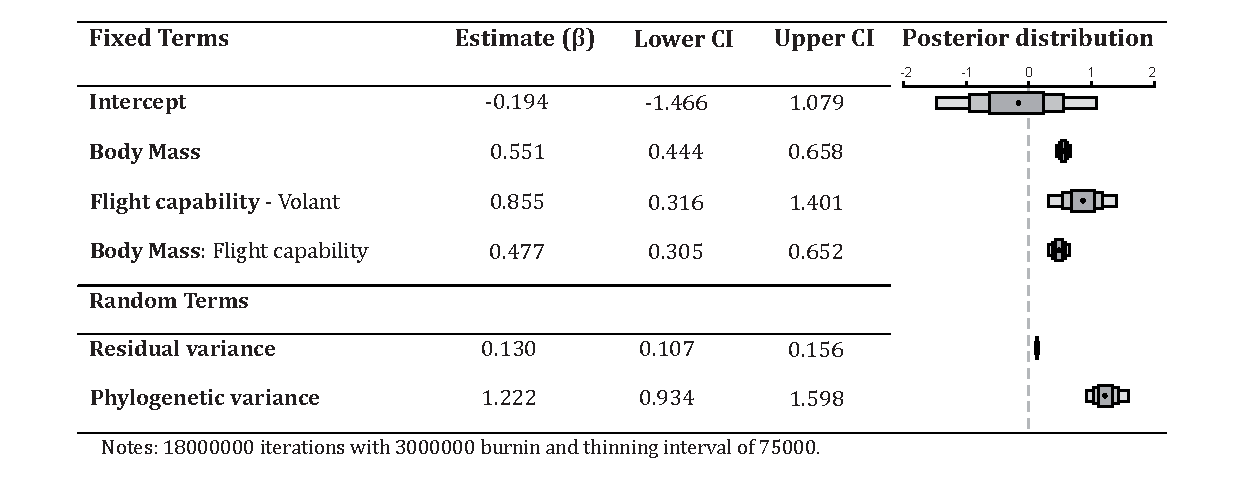
\includegraphics[width=\linewidth]{ch3-longevity-appendix/Table_B2.pdf}
\end{table}


\begin{table}[h]
  \caption[ ]{Table B3: Relationship between maximum longevity (years), body mass (g), foraging environment and activity period, in 536 species of volant birds and mammals with over 100 samples of longevity.}
  \label{tbl:Table B3.}
  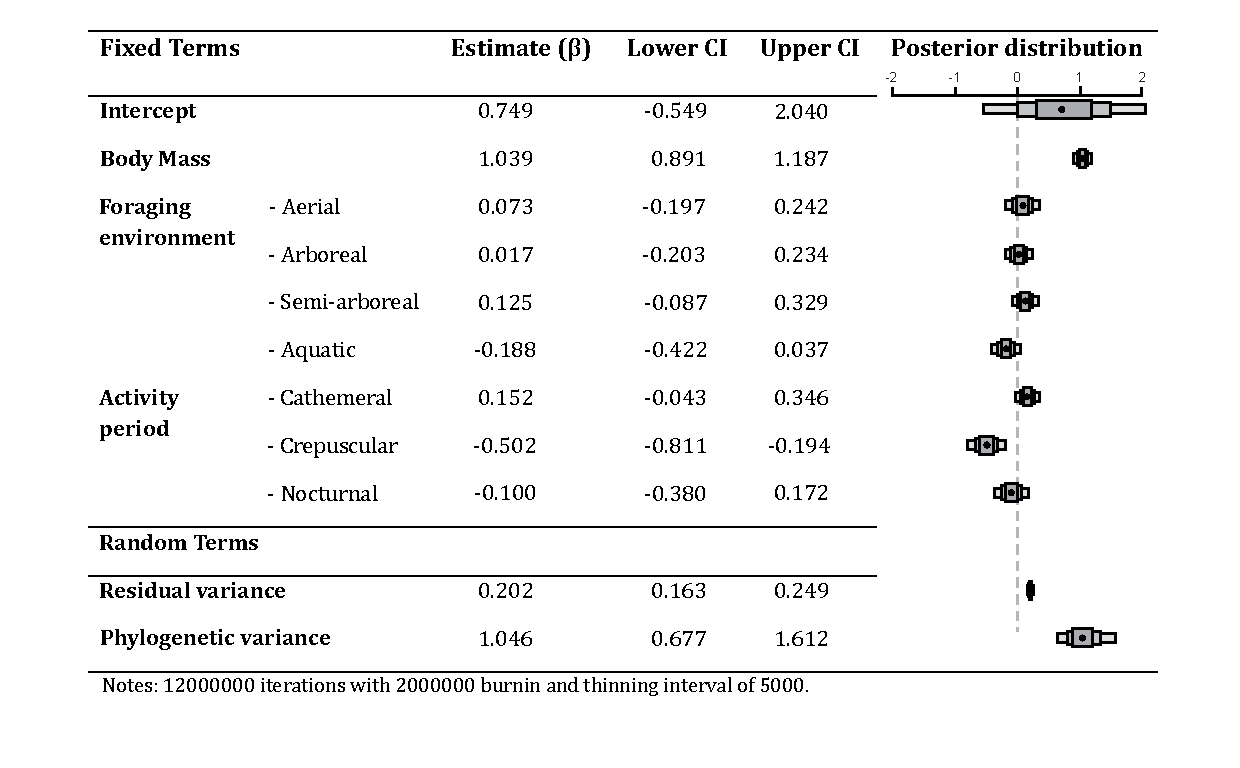
\includegraphics[width=\linewidth]{ch3-longevity-appendix/Table_B3.pdf}
\end{table}


\begin{table}[h]
  \caption[ ]{Table B4: Relationship between maximum longevity (years), body mass (g), foraging environment, fossoriality and activity period, in 373 species of nonvolant birds and mammals with over 100 samples of longevity.}
  \label{tbl:Table B4.}
  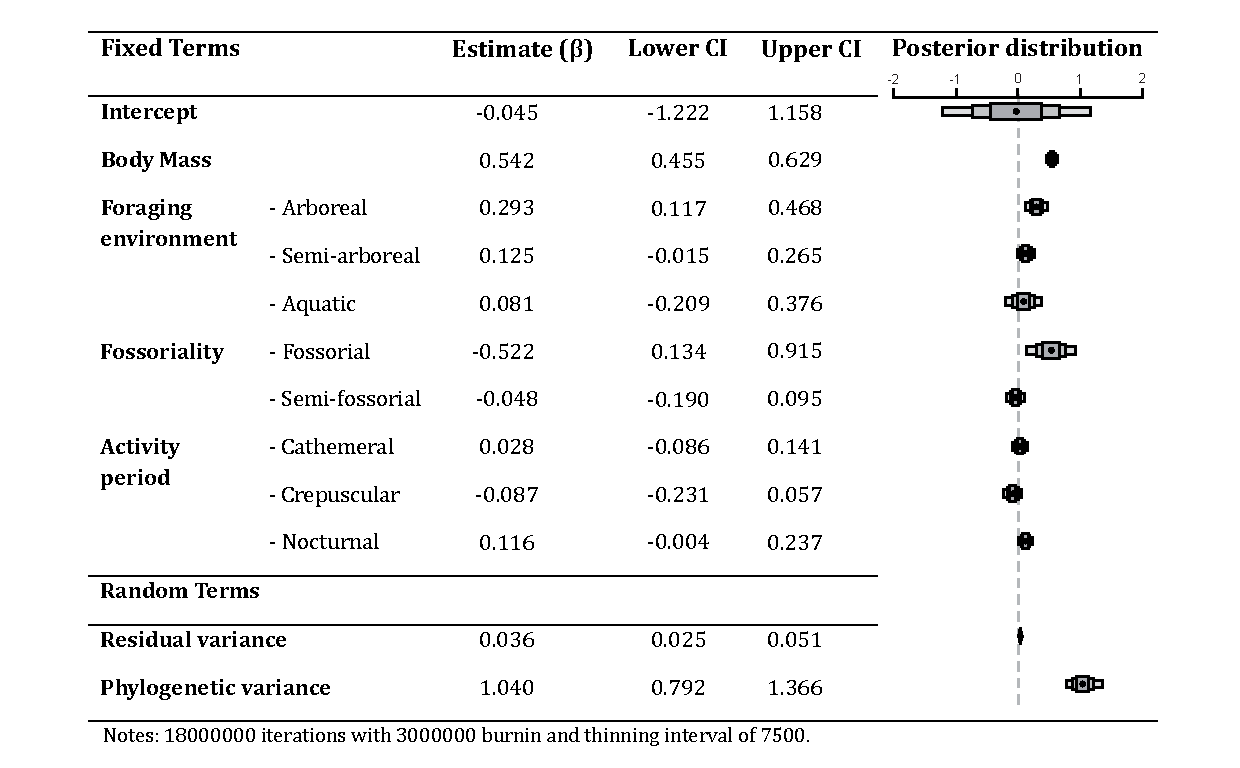
\includegraphics[width=\linewidth]{ch3-longevity-appendix/Table_B4.pdf}
\end{table}



\begin{table}[h]
  \caption[ ]{Table B5: Relationship between maximum longevity (years), body mass (g), foraging environment and activity period in 589 birds.}
  \label{tbl:Table B5.}
  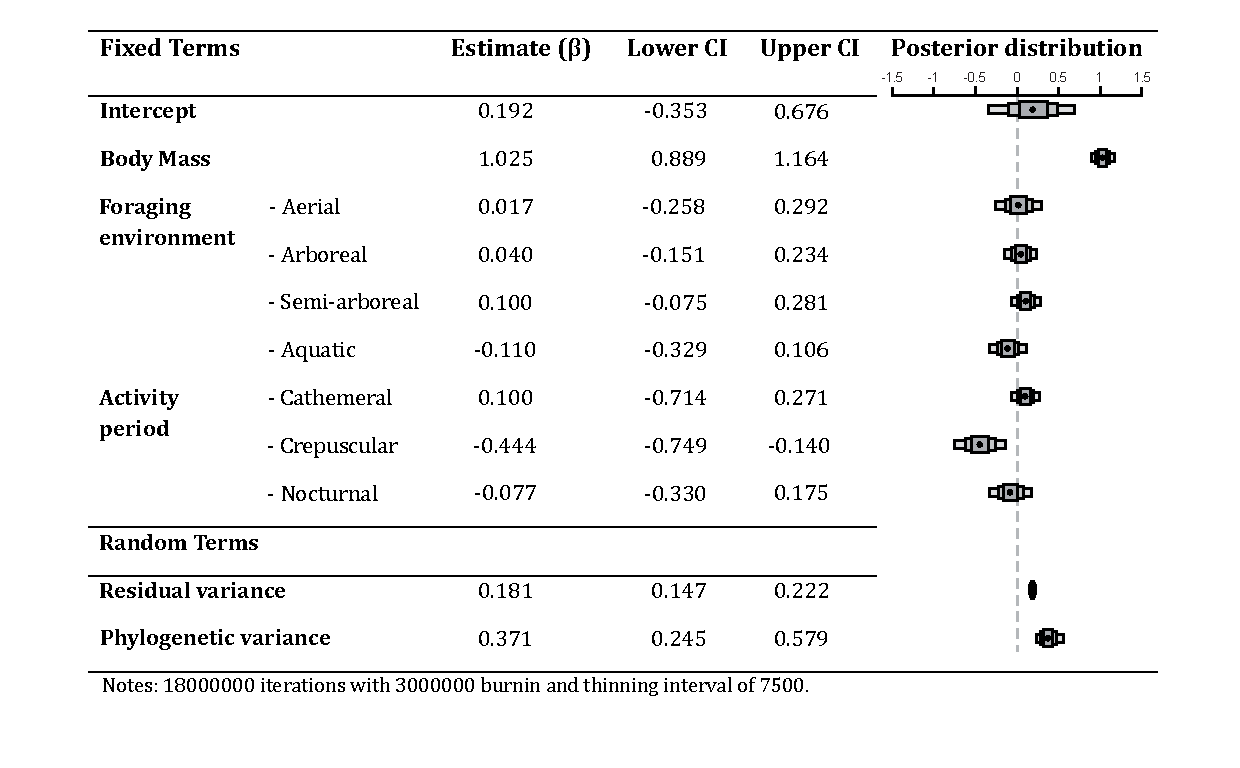
\includegraphics[width=\linewidth]{ch3-longevity-appendix/Table_B5.pdf}
\end{table}


\begin{table}[h]
  \caption[ ]{Table B6: Relationship between maximum longevity (years), body mass (g), foraging environment, fossoriality, and activity period 779 mammals..}
  \label{tbl:Table B9.}
  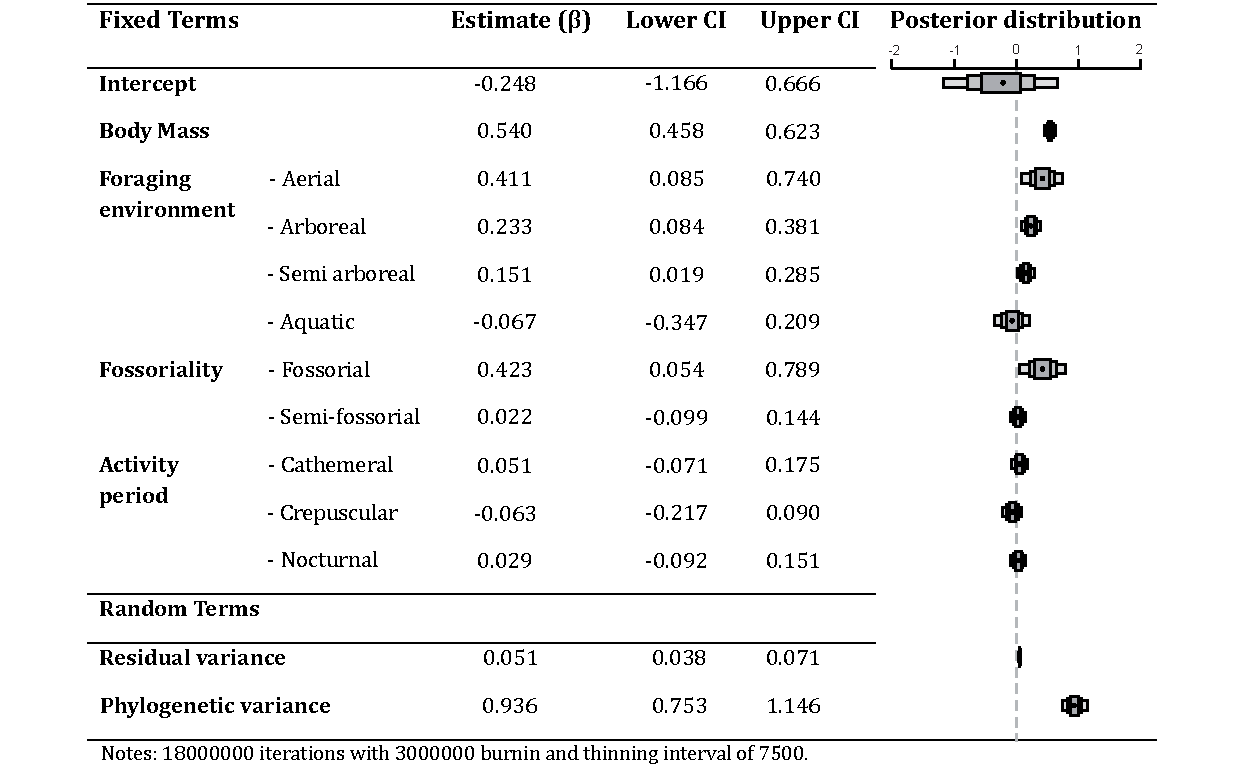
\includegraphics[width=\linewidth]{ch3-longevity-appendix/Table_B6.pdf}
\end{table}



%\bibliographystyle{PLoS-Biology}
%\bibliography{bibfile}

